\documentclass[12pt, openany]{book}

% This is all the packages and settings and so on.
% It is using custom fonts that needs to be installed on the computer. If they are not present, they have to be added manually.
\usepackage[
	citestyle=ieee, 
    bibstyle=ieee,
    style=numeric-comp,
    sorting=nty,
    maxbibnames=99, % Make sure we are printing all authors in the appendix
    ]{biblatex}
    
% Makes the last name first in the bibliography.
% \DeclareNameAlias{author}{last-first}
\DeclareNameAlias{author}{family-given}
    
% Specify the margins. This is 6.25inches in text with which 
% can be used to size figures to the correct size.
\usepackage[a4paper, margin=2.5625cm]{geometry}

\usepackage{eso-pic}					% Packages for layout and graphics 
\usepackage{graphicx}
\usepackage{tikz}
\usetikzlibrary{fadings}
\usepackage{setspace}
% \usepackage{tocloft}		 			% Fixing a bug with page style changes for toc
% \tocloftpagestyle{plain}
\usepackage{etoc} 						% Separate tocs for appendix and the rest    
\usepackage{chngcntr}					% Count figures within chapters
\usepackage{booktabs}					% Table formatting
\usepackage{fancyhdr}					% Setting the style for header and footer.
\usepackage{tabularx}
\usepackage{multirow}                   % For better tables 
\usepackage[hidelinks]{hyperref}		% Clickable links
\usepackage{nameref}					% References with names
\usepackage[parfill]{parskip}			% New line instead of indent for sections
\usepackage{tcolorbox}					% Create boxes around content
\tcbset{colback=white,arc=0mm}

\usepackage{amsmath}
\usepackage{mathdots}
\usepackage{yhmath}
\usepackage{siunitx}
\usepackage{array}
\usepackage{gensymb}
\usepackage{amssymb}
\usepackage{mathtools}              % Add text to math arrows.

\usepackage{cancel}
\usepackage{color}
\usepackage{multirow}
\usepackage{textcomp}               % Fixing warning for gensyb \perthousand
\usepackage{svg}                    % including svg files
\usepackage{caption}                % For subfigures
\usepackage{subcaption}
\usepackage{sectsty}
\usepackage{tocloft}

\usepackage{graphicx}
\usepackage{wrapfig}

\usepackage[printonlyused]{acronym}


\counterwithin{figure}{section} 
\counterwithin{table}{section}


% Remove the title and make sure that the text is adjusted
% \usepackage{abstract}
% \setlength{\absleftindent}{0mm}
% \renewcommand{\abstractname}{\vspace{-\baselineskip}}
% \renewcommand{\abstractnamefont}{\sffamily\fontsize{14}{15}}
% \renewcommand{\abstracttextfont}{\normalfont\fontsize{12}{13}}

% Renaming and setting style of table of contents
\renewcommand*\contentsname{Contents}
\renewcommand*\cfttoctitlefont{\fontsize{16}{0}\bf\sffamily}
\renewcommand\cftchapfont{\fontsize{14}{0}\bf\sffamily}
\renewcommand\cftchappagefont{\fontsize{13}{0}\bf\sffamily}
\renewcommand\cftsecfont{\fontsize{12}{0}\sffamily}
\renewcommand\cftsecpagefont{\fontsize{12}{0}\sffamily}
\renewcommand\cftsubsecfont{\fontsize{12}{0}\sffamily}
\renewcommand\cftsubsecpagefont{\fontsize{12}{0}\sffamily}

% Styling the header and footer
\fancyhf{}
\fancyhead{}
\fancyfoot{}
\fancyhead[L]{\fontsize{11}{10}\selectfont\leftmark}
\fancyfoot[R]{\footerfont\thepage}
\setlength{\headheight}{15.5pt}


\fancypagestyle{plain}{
    \fancyhf{}
    \fancyhead{}
    \fancyfoot{}
    \renewcommand{\headrulewidth}{0pt}
    \fancyfoot[R]{\footerfont\thepage}
}

\pagestyle{fancy}

% Making the command for placing text in random locations
\newcommand\PlaceText[3]{%
\begin{tikzpicture}[remember picture,overlay]
\node[outer sep=0pt,inner sep=0pt,anchor=south west] 
  at ([xshift=#1,yshift=-#2]current page.north west) {#3};
\end{tikzpicture}%
}

% Disable hyphenation
\pretolerance=10000
\tolerance=2000 
\emergencystretch=50pt


% Defining files for bibliography
%\addbibresource{ref.bib}
\addbibresource{references.bib}
% Add a second bibliography file for the second author to allow
% both to update it through the mendeley integration.
% \addbibresource{ref-author-2.bib}

% Defining document information
\title{Optimisation of parallel KD-trees using heuristics for neuron touch detection task}
\author{Daniel Benedí García}

\begin{document}
\setstretch{1.4}

% The front page of the document
\pagenumbering{roman}
\makeatletter
\begin{titlepage}

\vspace*{-4.6\baselineskip}
\hspace*{-0.15\textwidth}
\includegraphics[width=0.2\paperwidth]{setup/img/kth-logo.jpg}
\par\vspace*{2.5\baselineskip}

\PlaceText{65mm}{12mm}{\fontsize{12}{0}\sffamily DEGREE PROJECT IN TECHNOLOGY,}
\PlaceText{65mm}{17mm}{\fontsize{12}{0}\sffamily FIRST CYCLE, 15 CREDITS}
\PlaceText{65mm}{22mm}{\fontsize{12}{0}\sffamily\itshape STOCKHOLM, SWEDEN \the\year}

~\\

\makebox[0pt][l]{%
\begin{minipage}[b]{0.25\textwidth}
~\\
\end{minipage}
\begin{minipage}{0.65\textwidth}
\begin{flushleft}
{\fontsize{28}{24}\bf\sffamily\@title\\}
\vspace{1cm}
{\fontsize{16}{18}\bf\sffamily \@author}\\
\end{flushleft}
\end{minipage}
}


% \hspace*{-3cm}\begin{minipage}[b]{63.5mm}
% ~\\
% \end{minipage}
% \begin{minipage}{0.65\textwidth}
% \begin{flushleft}
% {\fontsize{28}{24}\bf\sffamily\@title\\}
% \vspace{0.5cm}
% {\fontsize{19}{17}\bf\sffamily \subtitle\\}
% \vspace{0.5cm} 
% {\fontsize{16}{0}\sffamily \@author}\\
% \end{flushleft}
% \end{minipage}


\AddToShipoutPictureBG*{%]
    \AtPageLowerLeft{%
        
\includegraphics[width=1.0\paperwidth]{setup/img/kth-footer.png}
    }%
}

\PlaceText{70mm}{280mm}{\color{white}\fontsize{12}{0}\sffamily KTH ROYAL INSTITUTE OF TECHNOLOGY }
\PlaceText{70mm}{285mm}{\color{white}\fontsize{8}{0}\sffamily ELECTRICAL ENGINEERING AND COMPUTER SCIENCE }
\end{titlepage}
\makeatother

\newpage
\newpage
\thispagestyle{plain}
~\\
\begin{minipage}[b]{0.25\textwidth}
~\\
\end{minipage}
\begin{minipage}{0.65\textwidth}
\begin{flushleft}
{\fontsize{28}{24}\bf\sffamily Optimisation of parallel KD-trees using heuristics for neuron touch detection task\\}
\vspace{3cm}
{\fontsize{16}{18}\sffamily Daniel Benedí García}\\
\end{flushleft}
\end{minipage}
\vfill
{ \setstretch{1.1}
	\subsection*{Degree Project in Computer Science}
	Date: \\
	Supervisor: Alexander Kozlov \\
	Examiner: \\
	School of Electrical Engineering and Computer Science \\
	Swedish title: \\
	~
}


\newpage
\thispagestyle{plain}
%%%%%%%%%%%%%%%%%%%%%%%%%%%%%%%%%%%%
%%  The English abstract          %%
%%%%%%%%%%%%%%%%%%%%%%%%%%%%%%%%%%%%
\chapter*{Abstract}
%%%%%%%%%%%%%%%%%%%%%%%%%%%%%%%%%%%%
Write an abstract. Introduce the subject area for the project and describe the problems that are solved and described in the thesis. Present how the problems have been solved, methods used and present results for the project. Use probably one sentence for each chapter in the final report.

The presentation of the results should be the main part of the abstract. Use about ½ A4-page.
English abstract


\newpage
\thispagestyle{plain}
%%%%%%%%%%%%%%%%%%%%%%%%%%%%%%%%%%%%
%%	 The Swedish abstract         %%
%%%%%%%%%%%%%%%%%%%%%%%%%%%%%%%%%%%%
\chapter*{Abstract}
%%%%%%%%%%%%%%%%%%%%%%%%%%%%%%%%%%%%
Svenskt abstract
Svensk version av abstract – samma titel på svenska som på engelska.

Skriv samma abstract på svenska. Introducera ämnet för projektet och beskriv problemen som löses i materialet. Presentera


\newpage
\thispagestyle{plain}
\chapter*{Acknowledgements}
Write a short acknowledgements. Don't forget to give some credit to the examiner and supervisor.

\newpage

\etocdepthtag.toc{mtchapter}
\etocsettagdepth{mtchapter}{subsection}
\etocsettagdepth{mtappendix}{none}
\thispagestyle{plain}
\tableofcontents

\newpage




\pagenumbering{arabic}

\chapter{Introduction}

Provide a general introduction to the area for the degree project. Use references!

Link things together with references. This is a reference to a section: \ref{sec:background}.

\section{Background}
\label{sec:background}
Present the background for the area. Give the context by explaining the parts that are needed to understand the degree project and thesis. (Still, keep in mind that this is an introductory part, which does not require too detailed description).

Use references\footnote{You can also add footnotes if you want to clarify the content on the same page.}

Detailed description of the area should be moved to Chapter 2, where detailed information about background is given together with related work. 

This background presents background to writing a report in latex.


Example citation \cite{Jones2017} or for two authors: \cite{Jones2017, Liu2017}

Look at sample table \ref{tab:sample-table-label} for a table sample.

\begin{table}[!ht]
\centering
\caption{Sample table. Make sure the column with adds up to 0.94 for a nice look.}
~\\
\label{tab:sample-table-label}
\begin{tabular}{p{0.3\textwidth} p{0.64\textwidth}}
\toprule
\textbf{SAMPLE}		  & \textbf{TABLE}                                                                                                                                                  \\ \toprule
One                   & Stuff 1 \\
\midrule
Two                   & Stuff 2 \\
\midrule
Three                 & Stuff 3\\
\bottomrule
\end{tabular}
\end{table}



Boxes can be used to organize content

\begin{tcolorbox}[title={Development environment for prototype}]
	\tt{
		\textbf{Operating systems }\\
		computer: Linux - kernel 4.18.5-arch1-1-ARCH\\
		android phone: 8.1.0\\
		~\\
		\textbf{Build tools}\\
		exp (build tool): version 55.0.4\\
		~\\
		...
	}
\end{tcolorbox}

\section{Problem}
Present the problems found in the area. Preferable use and end this section with a question as a problem statement. 

Use references
Preferable, state the problem, to be solved, as a question. Do not use a question that can be answered with yes and/or no. 

Use acronyms:
The \ac{CPU} is very nice. It is a \ac{CPU}

\section{Purpose}
The purpose of the degree project/thesis is the purpose of the written material, i.e., the thesis. The thesis presents the work / discusses / illustrates and so on.

It is not “The project is about” even though this can be included in the purpose. If so, state the purpose of the project after purpose of the thesis).

\section{Goal}
The goal means the goal of the degree project. Present following: the goal(s), deliverables and results of the project. 

\section{Benefits, Ethics and Sustainability}
Describe who will benefit from the degree project, the ethical issues (what ethical problems can arise) and the sustainability aspects of the project.

Use references!

\section{Methodology}
Introduce, theoretically, the methodologies and methods that can be used in a project and, then, select and introduce the methodologies and methods that are used in the degree project. Must be described on the level that is enough to understand the contents of the thesis. 

Use references!

Preferably, the philosophical assumptions, research methods, and research approaches are presented here. Write quantitative / qualitative, deductive / inductive / abductive. Start with theory about methods, choose the methods that are used in the thesis and apply. 


Detailed description of these methodologies and methods should be presented in Chapter 3. In chapter 3, the focus could be research strategies, data collection, data analysis, and quality assurance.


\section{Stakeholders}
Present the stakeholders for the degree project.

\section{Delimitations}
Explain the delimitations. These are all the things that could affect the study if they were examined and included in the degree project. 
Use references!

\section{Outline}
In text, describe what is presented in Chapters 2 and forward. Exclude the first chapter and references as well as appendix. 

\chapter{Background}
\label{chapter:background}

\section{Neuronal morphology}
Neurons are the fundamental units of the nervous system.  There are different types of neurons depending on their function, shape and other factors. If we classify by function, there are three types: sensory neurons, motor neurons and interneurons. The sensory neurons respond to stimuli and send signals to the spinal cord or brain. The motor neurons receive information from the brain and spinal cord to control everything, like muscles or glands. Interneurons connect other neurons within the same region. A neural circuit or neuronal network is multiple neurons connected.
\begin{wrapfigure}{r}{0.25\textwidth}
    \centering
    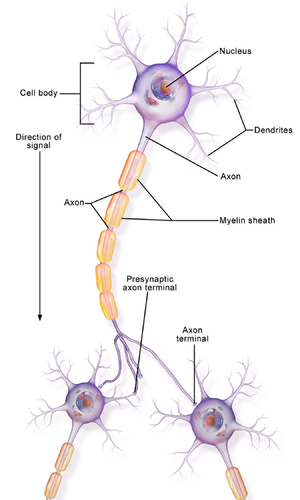
\includegraphics[width=0.25\textwidth]{setup/img/NeuronParts.png}
    \caption{A sketch of how a neuron may look like \cite{wiki:interneurons}}
    \label{fig:NeuronParts}
\end{wrapfigure}

In physiology, a neuron consists of a cell body or soma with the nucleus, dendrites and axon, as seen in the figure \ref{fig:NeuronParts}. The soma is a compact structure, whereas the axon and dendrites are filaments from the soma. Typically a dendrite receives signals from other neurons and the axon transmits information to other neurons. The cell body, soma, is where the nucleus lies and where proteins are made to be transported throughout the axon and dendrites.

A point where the distance between two neurons is lower than a certain threshold defines a touchpoint. If there is a touchpoint, then a synapse can emerge. A synapse is a structure that permits a neuron to pass an electrical or chemical signal to another neuron. There are different types of synapses. The most common is axodendritic. But there are also other types, depending on which parts of the neurons are in touch, such as axo-axonic (axon with axon), dendro-dendritic (dendrite with dendrite), axo-secretory (axon to bloodstream), somatodendritic (soma to dendrite), dendro-somatic (dendrite with soma), and somato-somatic (soma with soma) synapses. A neuron can have up to 6000 synapses with neighbouring neurons\cite{Sherwood2020}.

\section{Simulation of local neuronal network}
The usual workflow in research consists of three main steps: single-cell morphology reconstruction, building a local network and simulating the signals exchange.

The single-cell morphology reconstruction consists of retrieving the neurons' morphology to simulate. To do so, first, the bunch of neurons need to be separated to be able to do a reconstruction of the morphology of the neurons and a classification. Also, a repairing phase is necessary because there could have been errors in previous steps. This process ends up with isolated single-cell models. There are different databases with reconstructions of neuron morphologies, both private and public access, but the most common and huge is \href{https://neuromorpho.org/}{NeuroMorpho.Org} \cite{Neuromorpho1,Neuromorpho2}.

The network building step is computationally more intensive because there is a large number of points in the space where a lot of spatial calculations are involved. First, the single-cell models are cloned, transformed and translated to their final position. Then, all the touching points between the neurons need to be found. This task has a higher computational cost because it implies checking almost all the points of the neurons against all the compartments of the other neurons. Finally, the synapses are established according to geometric and biological restrictions.

Finally, simulating the signal exchange of the neurons relies on different software tools such as NEURON \cite{carnevale2006neuron}, Arbor \cite{8671560}, Brian \cite{Stimberg2019} and IBM Neural Tissue Simulator \cite{10.3389/fninf.2011.00015}. These programs allow the simulation of detailed biophysical models from single-cell models to large-scale networks.

\section{Space-partition data structures}
Space partitioning is the process of dividing a space into disjoint subsets, non-overlapping. The division can be done in two or more regions, and any point can then lie in only one subregion. Space partitioning is often hierarchical, which means the subsets are also divided recursively into other areas. The recursive division allows the organization of the subsets into a tree called a space-partitioning tree. 

The space-partitioning trees can divide the subsequent space into several regions each time or just two each iteration. When splitting the area into only two subregions, it is called binary space partitioning (BSP) tree. BSP trees usually use a hyperplane, a generalization of the plane for higher dimensions, to divide space, so the points on each side of the hyperplane form each subregion.

There is also another kind of tree that not only does it divides the space but also the time. For example, the TPR*-tree \cite{TPRtree}, but they are out of the scope of this thesis.

\subsection{Octree}
\begin{wrapfigure}{r}{0.5\textwidth}
    \centering
    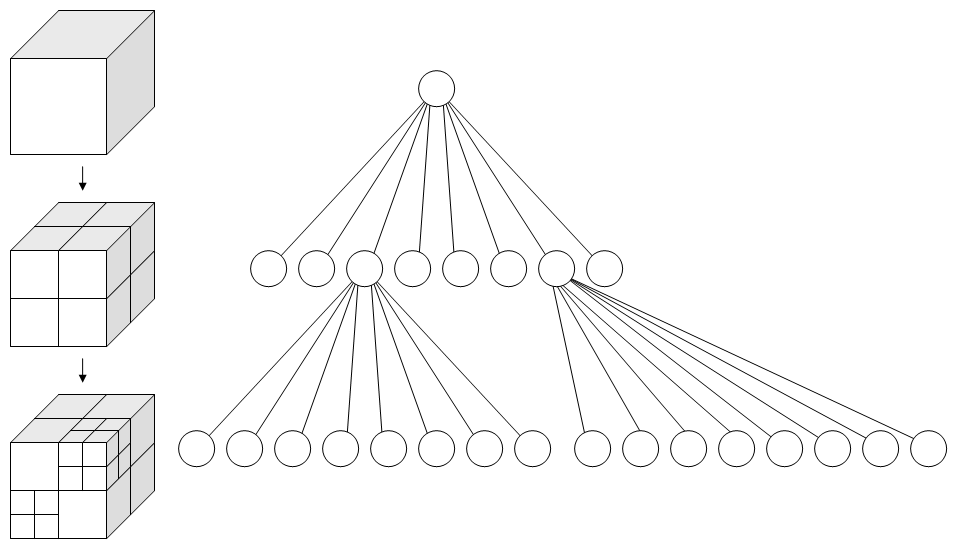
\includegraphics[width=0.5\textwidth]{setup/img/Octree.png}
    \caption{Left: Recursive subdivision of a cube into octants. Right: The corresponding octree. \cite{wiki:octree}}
    \label{fig:octree}
\end{wrapfigure}
An octree is a data structure to generate partitions of a 3D space. Each node has exactly eight children, except the leaves. There are two types of octree: point region (PR) octree and matrix-based (MX) octree. In a PR octree, the node represents one three-dimensional point, which is the centre of the subdivision, and it is one of the corners of the eight children. In an MX octree, the division point is implicitly the centre of the space. The root node of a PR octree represents infinite space, while in an MX octree, it represents a finite bounded space. When can see an example in the figure \ref{fig:octree}.

This data structure was proposed by Donald Meagher in 1980 \cite{Octree} and the construction goes as follows. First, it divides the current 3D volume into eight boxes. If any box has more than one point then apply again the algorithm. If the box has zero or one point, stop building that branch.

\subsubsection{Quadtree}
A quadtree is another tree data structure proposed earlier by Raphael Finkel and Joun Louis Bentley in 1974 \cite{Quadtree}. This data structure is the two-dimensional version of the Octree. Similar to the Octree, the algorithm divides the 2D space into four quadrants recursively. No more detail is needed for this data structure because our data is 3D-based and this solution works for 2D points.

\subsection{R-tree}
\begin{wrapfigure}{r}{0.5\textwidth}
    \centering
    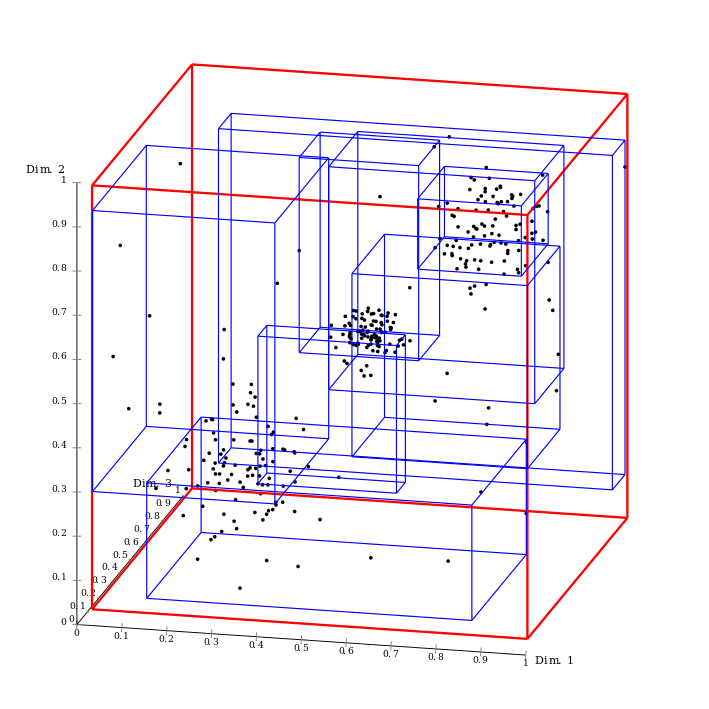
\includegraphics[width=0.5\textwidth]{setup/img/RTree-Visualization-3D.png}
    \caption{Visualization of an R*-tree for 3D points \cite{wiki:rtree}}
    \label{fig:rtree}
\end{wrapfigure}
An R-tree is a data structure used for spatial access methods for k-dimensional data. Antonin Guttman proposed the R-tree in 1984 \cite{10.1145/971697.602266} and the key idea is to group nearby points under a tight bounding box. The construction of the tree is button-up, which means the leaves are constructed first and it starts associating nodes with their bounding boxes until the root is reached. One visualization of the space partition made by an R-tree in a three-dimensional space can be seen in the figure \ref{fig:rtree}

This tree has different variations like priority R-tree, R$^*$-tree, R$^+$ tree, RR$^*$-tree, Hilbert R-tree and X-tree. One common variation used in the touching point problem is R*-tree. This variant has a slightly higher construction cost, but on the other hand, it will have a lower cost while querying. The main difference between R$^*$-tree and R-tree is that R$^*$-tree reduces the overlapping of subtrees, pruning more branches while querying and improving the performance, therefore. 

\pagebreak
\subsection{$k$-d trees}
\begin{wrapfigure}{r}{0.5\textwidth}
    \centering
    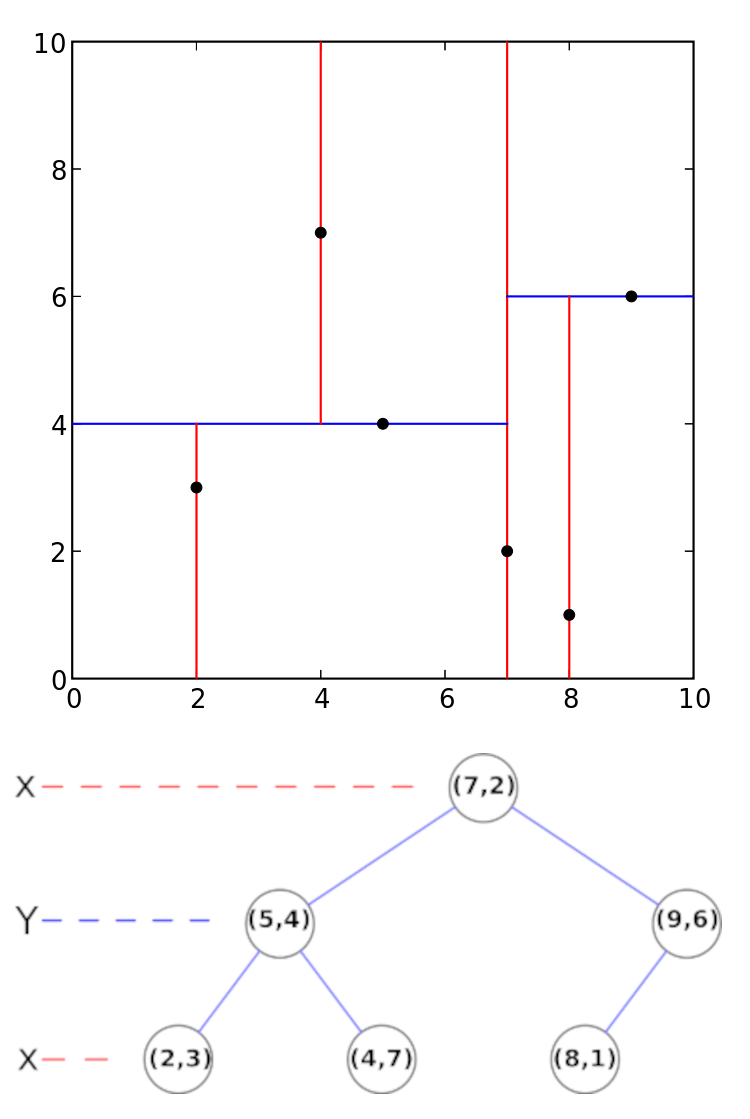
\includegraphics[width=0.5\textwidth]{setup/img/kdtree.png}
    \caption{k-d tree decomposition for a point set \cite{wiki:kdtree}}
    \label{fig:kdtree}
\end{wrapfigure}
$k$-d tree is a data structure for space-partitioning $k$-dimensional points. It is a characteristic case of space partitioning trees called binary space partitioning (BSP) trees. Being a BSP tree means that each time it splits the space it is done in two convex subsets. It was proposed in 1975 by Jon Louis Bentley \cite{Bentley}. The construction of the $k$-d tree is done recursively. First of all, one point and one axis are selected. Originally, the dimension was chosen by round-robin and the point was chosen by the median in that axis, but in this thesis, we will explore some other options. The axis and the point will form a hyperplane aligned with the axis. Then, the algorithm splits the points into two subsets: the point at the "left" of the plane and the points at the "right". Finally, the left and right subtrees are constructed using the same algorithm. One example of the execution of this algorithm can be seen in the figure \ref{fig:kdtree}.

\section{Previous research}
There are several studies on spatial-partitioning structures, but a little few focus on the touch detection problem. In their thesis, Adamsson and Vorkapic \cite{Adamsson_Vorkapic_2016} analyze the performance of different spatial-partitioning structures: $k$-d trees, vantage-point trees and octrees. They discovered that vantage-point trees are the best option with small populations, but $k$-d trees work better with larger networks. Because of their result, we choose $k$-d trees over other data structures. In Beredent and Brask's thesis \cite{Brask_Berendt_2020}, they analyze the memory efficiency for R-trees and R$^*$-trees. They analyzed the performance with realistic neuron densities and found out that R$^*$-tree has the same good scalability properties as $k$-d trees.

Compared with the studies on spatial-partitioning structures on the touch detection problem,  more studies are trying to optimize the $k$-d trees partition for different applications, such as computer graphics or curve analysis. Hu, Nooshabadi and Ahmadi in their paper \cite{LinjiaSaeidMajid} propose a method for constructing $k$-d trees and doing nearest neighbor search (NNS) with a speed up of a factor of 30, compared with a serial CPU. Wald and Havran \cite{WaldHavran06} propose an heuristic for choosing the dimension and splitting point called surface area heuristic that will speed up for raytracing with objects based on triangles. In other paper by different authors \cite{Yucheng}, they propose a heuristic called Curve Complexity Heuristic, which aim is to allow the exploration of 3D curves based on the neighbourhood.
\chapter{Methods}
\label{chapter:methods}
% \thispagestyle{fancy}

\section{Reconstruction of a neuronal network}
\label{reconstruction}
First of all, we chose to reconstruct the neuronal network based on a single neuron, a fast-spiking interneuron. \href{https://neuromorpho.org/}{NeuroMorpho.Org} \cite{Neuromorpho1,Neuromorpho2} is an archive containing multiple reconstructions of different types of neurons from across different researches. The choice was completely arbitrary and was made to simplify the biological complexity of the problem while keeping the computational complexity because fast-spiking interneurons allow the creation of any kind of synapse. The exact neuron was "NMO\_36576" from one research of 2013 \cite{interneuron}, the figure \ref{fig:interneuron} contains a representation of this neuron. This specimen belonged to the subiculum of a rat and one characteristic of note is that the neuron spatial distribution is not uniformed, $298.75 \mu m$ x $538.69 \mu m$ x $66.28 \mu m$.
\begin{figure}[h!]
    \centering
    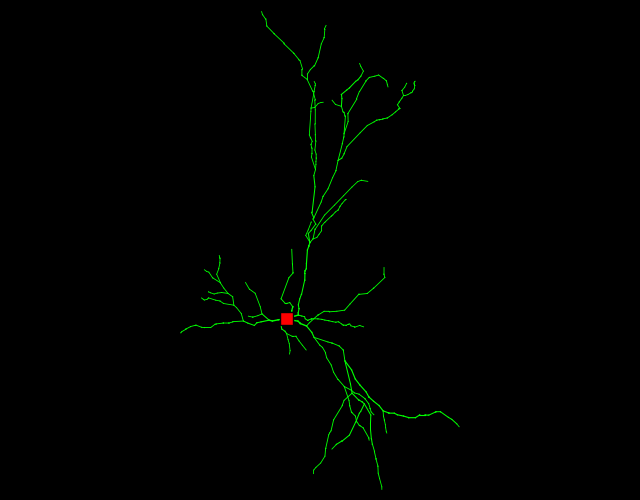
\includegraphics[width=0.75\textwidth]{figures/interneuron.png}
    \caption{Fast-spiking interneuron used in the thesis.}
    \label{fig:interneuron}
\end{figure}

To avoid reading the SWC file every time that it was needed to replicate the neuron, it was designed another file called RPL. This new format file defined a neuron per line and each line contained which transformations were going to be applied. The possible transformations defined were rotation and translation. Scaling and shearing were discarded because they deform the morphological definition of the neuron. A transformation was defined by three values: the first value defined which transformation (0 for translation and 1 for rotation), the second value defined which axis (0 means axis x, 1 means axis y, 2 means axis 3) and the third value defined the amount of transformation in micrometres for translation and radians for rotation. Any amount of transformation could be concatenated, so every possible neuron was possible.

\section{Data structure and construction algorithm}
\subsection{$k$-d tree}
When building a $k$-d tree are necessary a list of the points and a depth. As shown in algorithm \ref{alg:buildtree}, if the list of nodes is empty, we have finished building the tree and it is none. Otherwise, it first needs to find the dimension along which the splitting plane (or hyperplane) is going to be defined and then it chooses a point to create the plane (or hyperplane). Then, the algorithm divides the space into two subsets that are at the left or the right of the plane (or hyperplane) along that dimension. Finally, it creates the subtrees recursively increasing the depth by one. The returned node needs to contain not only the point and the left and right subtree but also the splitting dimension, so when performing a spatial-query, it is possible to know which dimension is responsible for the branches. 
\begin{algorithm}[h!]
    \caption{Constructs a $k$-d tree
        \label{alg:buildtree}}
    \begin{algorithmic}[1]
    \Require{$N$ is the list of points to construct the $k$-d tree with.}
    \Require{$k$ is the depth of the $k$-d tree.}
    \Statex
    \Function{BuildTree}{$N, k$}
        \If{$|N| = 0$}
            \State \Return{nullptr}
        \EndIf
        \State $d$, $p$ $\gets$ SplittingFunction($N, k$) \Comment{$d$ is the splitting dimension and $p$ is the point}
        \State LeftSplit  $\gets \{ n \in N\, |\, n_d \leq p_d \land n \neq p \} $ 
        \State RightSplit $\gets \{ p \in N\, |\, p_d   <  n_d \land n \neq p \} $ 
        \State LeftChild  $\gets$ \Call{BuildTree}{$LeftSplit, k+1$}
        \State RightChild $\gets$ \Call{BuildTree}{$RightSplit, k+1$}
        \State \Return{new \Call{Node}{$p$,$d$,LeftChild,RightChild}}
    \EndFunction
    \end{algorithmic}
\end{algorithm}

\pagebreak

\section{Splitting function and heuristics}
The canonical and original method for dividing the list of nodes is really simple and still leaves a lot of room for improvement. That is the reason because there are several studies trying to improve the splitting function for different applications. This thesis studied how the proposed splitting functions work for the touching point detection.

\subsection{Canonical splitting function}
The canonical method was first described whit the $k$-d tree in its original paper \cite{Bentley}. This method selects the splitting dimension by round-robin, that means the dimension cycles along all the axis. For example, in a 3D tree, the first plane will be aligned with the x-axis, the root's children will both have y-aligned planes, the grandchildren's planes will be aligned with the z-axis, the root's great-grandchildren will all have x-aligned planes, and so on. Once the axis is chosen, the algorithm chooses the median point in that axis from all the points. One possible implementation of this algorithm is the algorithm \ref{alg:canonical}.
\begin{algorithm}[h!]
    \caption{Canonical splitting function
        \label{alg:canonical}}
    \begin{algorithmic}[1]
    \Require{$N$ is the list of points to construct the $k$-d tree with.}
    \Require{$k$ is the depth of the $k$-d tree.}
    \Require{$K$ is the number of dimensions.}
    \Statex
    \Function{SplittingFunction}{$N, k$}
        \State axis $\gets \pmod{K}$ 
        \State \textbf{select} median \textbf{by} axis \textbf{from} N
        \State \Return{(axis,median)}
    \EndFunction
    \end{algorithmic}
\end{algorithm}

The main advantage of this method is that it leads to a balanced $k$-d tree, that means that each leaf of the tree is approximately at the same distance to the root. Selecting the median is a complex task were different approaches can be done. Sorting all the points with a sorting algorithm such as heapsort or mergesort, will lead into a complexity $\mathcal{O}(n\log{}n)$. An improved solution with complexity $\mathcal{O}(n)$ called PICK \cite{BLUM1973448} can be also implemented. A common implementation that is approximate selects random points from the total of points and use the median of those points. Although it is not optimal and does not ensure a balanced tree, it is widely used and often results in nicely balanced trees. In this thesis, we have used a built-in function from C++11 called "std::nth\_element". It is a partial sorting algorithm that rearranges the elements in the vector such as the element pointed at by the $n^{th}$ is changed so it would occur in that position if the vector was sorted, all elements before are less than or equal to the new $n^{th}$ element and the complexity is linear to the number of elements $\mathcal{O}(n)$ \cite{C++11iso}.

\subsection{Surface area heuristic}
The surface area heuristic (SAH) was proposed by MacDonald and Booth in their paper of 1990 \cite{MacDonald1990-jo}. The main idea behind their proposal is that the number of rays likely to intersect a convex object is roughly proportional to its surface area, assuming that the ray origins and directions are uniformly distributed throughout the space. We believed there was a similarity with our task because our neurons are uniformly distributed in the space, and the orientation of the touching point does not matter, so it can be said that the "ray direction" is also evenly distributed. Instead of using the straight-forward implementation from the original description of the algorithm that is $\mathcal{O}(n^2)$ for building the tree, we have used other implementation \cite{WaldHavran06} that is $\mathcal{O}(n \log^2{}n)$. This implementation is the algorithm \ref{alg:sah}.
\begin{algorithm}[h!]
    \caption{Surface area heuristic
        \label{alg:sah}}
    \begin{algorithmic}[1]
    \Require{$N$ is the list of points to construct the $k$-d tree with.}
    \Require{$k$ is the depth of the $k$-d tree.}
    \Require{$K$ is the number of dimensions.}
    \Statex
    \Function{SplittingFunction}{$N, k$}
        \State $\^{C}, \^{d}, \^{p} \gets (\infty, \infty, \emptyset)$
        \For{$i = 1..K$}
            \State $E \gets \emptyset$
            \ForAll{$p \in N$}
                \State $E \gets E \cup (p,p_i,+) \cup (p,p_i,-)$ \label{alg:sah:change}
            \EndFor
            \State \Call{sort}{$E$} \Comment{First, it orders by $p_i$ and if they are equal, then it goes first the $-$ and then the $+$}
            \State $N_l, N_p, N_r \gets (0,0,|N|)$
            \For{$j = 1..|E|$}
                \State $p \gets E_{j,p}$
                \State $p^{+},p^{-},p^{|} \gets 0$
                \While{$j < |E| \land E_{j,\xi} = p_\xi \land E_{j,type} = - $}
                    \State $p^{-} \gets p^{-} + 1$
                    \State $j \gets j + 1$
                \EndWhile
                \While{$j < |E| \land E_{j,\xi} = p_\xi \land E_{j,type} = |$}
                    \State $p^{|} \gets p^{|} + 1$
                    \State $j \gets j + 1$
                \EndWhile
                \While{$j < |E| \land E_{j,\xi} = p_\xi \land E_{j,type} = + $}
                    \State $p^{+} \gets p^{+} + 1$
                    \State $j \gets j + 1$
                \EndWhile
                \State $N_p \gets p^{|}$
                \State $N_r \gets N_r - p^{|} - p^{-}$
                \State $C \gets SAH(p,N_l,N_r,N_p)$ \label{alg:sah:sah}
                \If{$C < \^{C}$}
                    \State $\^{C}, \^{d}, \^{p} \gets (C, i, p)$
                \EndIf
                \State $N_l \gets N_l + p^{+} + p^{|}$
                \State $N_p \gets 0$
            \EndFor
        \EndFor
        \State \Return{$(\^{d},\, \^{p})$}
    \EndFunction
    \end{algorithmic}
\end{algorithm}

 The called function in line \ref{alg:sah:sah}, SAH, basically is defined as:
\begin{align*}
  SAH(p,N,N_l,N_r,N_p) = \lambda * (K_T + min(&\frac{(N_l+N_p)|\{t\in N\, |\, t_i < p_i\}|+N_r|\{t\in N\, |\, t_i > p_i\}|}{|N|},\\
  &\frac{N_l|\{t\in N\, |\, t_i < p_i\}|+(N_p+N_r)|\{t\in N\, |\, t_i > p_i\}|}{|N|}))
\end{align*}
There are two values in this function that are unknown $\lambda$ and $K_T$, $\lambda$ is a factor to prioritize cutting empty space, and it will be $0.8$ if $N_l$ or $N_r$ is $0$, otherwise it is $1$. $K_T$ is a constant that represents the cost of a transversal step in the tree. We stablished it to $0.2$ based on other paper \cite{Yucheng}. The implemented version is not exactly the proposed in the original article. In line \ref{alg:sah:change}, they firstly clamp the triangle containing the point and in case the resulting triangle is planar, then it changes what is added to $E$, by $E \cup (p, p'_{min,k}, |)$. We have done this because we are creating one $k$-d tree per neuron, so the neuron will always be inside the voxel of the $k$-d tree.


\subsection{Curve complexity heuristic}
The curve complexity heuristic propose a new splitting function based on SAH to optimize $k$-d trees for curves abstractions \cite{Yucheng}. The main idea behind their proposal is to adapt SAH so they can perform radius nearest curve search better. We believed there is a great similarity between their proposal and our problem because we also want to find all the nearest neurons given a query point $\mathbf{q}$ and a distance $\mathbf{r}$. A possible implementation could be the algorithm \ref{alg:cch}.
\begin{algorithm}[h!]
    \caption{Curve complexity heuristic
        \label{alg:cch}}
    \begin{algorithmic}[1]
    \Require{$N$ is the list of points to construct the $k$-d tree with.}
    \Require{$k$ is the depth of the $k$-d tree.}
    \Require{$K$ is the number of dimensions.}
    \Statex
    \Function{SplittingFunction}{$N, k$}
        \State $\^{C} \gets \infty$
        \State $\^{p} \gets \emptyset$
        \State $\^{d} \gets \emptyset$
        \For{i = 1..K}
            \State $C_i \gets 0$ \Comment{$C(T) = C_{\text{traversal}}(T)+C_{\text{backtrack}}(T)-nT_{\text{dist}}$}
            \State \textbf{select} median \textbf{by} axis \textbf{from} N
            \Statex
            \Comment{$C_{\text{trasversal}}(T) = T_{\text{trasversal}} + [P(T_l|T)l+P(T_r|T)r]T_{\text{dist}}$}
            \State $C_i \gets 0.2 + l*\frac{\text{Volume}(\{p \in N\, |\, p_i < \text{median}_i\})}{\text{Volume}(N)} + r*\frac{\text{Volume}(\{p \in N\, |\, p_i > \text{median}_i\})}{\text{Volume}(N)}$  
            
            \Comment{$C_{\text{backtracl}}(T) = \lambda(\log{\frac{1}{\rho}(n)+\log{\frac{1}{\tau}}(n)})/2$}
            \Comment{$\rho := \frac{l}{n}$, $\tau := \frac{r}{n}$}
            \State $C_i \gets C_i + \lambda*(\frac{\log{}(n)}{\log{}(\frac{|\{p \in N\, |\, p_i < \text{median}_i\}|}{|N|})} + \frac{\log{}(n)}{\log{}(\frac{|\{p \in N\, |\, p_i > \text{median}_i\}|}{|N|})})$
            \If{$C_i < \^{C}$}
                \State $\^{C} \gets C_i$
                \State $\^{p} \gets \text{median}$
                \State $\^{d} \gets i$
            \EndIf
        \EndFor
        \State \Return{$(\^{d},\, \^{p})$}
    \EndFunction
    \end{algorithmic}
\end{algorithm}

In their paper, they do not study the time complexity of their solution, so we are going to do it. Assuming that the volume functions and selecting the median are $\mathcal{O}(n)$ and the other operations are $\mathcal{O}(1)$. To obtain the cost function, it will sum the cost of finding the median ($n$), the find of the volumes function ($n$), the cost of splitting ($2n$) and the cost of constructing the subtrees recursively ($2T(\frac{n}{2})$):
\begin{align*}
    T(n) &= n + n + 2n + 2T(\frac{n}{2})\\
    &= 4n + 2T(\frac{n}{2}) \\
    &= 4n + 2[4\frac{n}{2} + 2T(\frac{n}{4})] = 8n + 4T(\frac{n}{4}) \\
    &= 8n + 4[4\frac{n}{4} + 2T(\frac{n}{8})] = 12n + 8T(\frac{n}{8}) \\
    &= 12n + 8[4\frac{n}{8} + 2T[\frac{n}{16}]] = 16n + 16T(\frac{n}{8}) \\
    &= \dots = 4*i*n + 2^iT(\frac{n}{2^i}), i \in \mathbb{Z}^+ \\
    &\text{This ends when $\frac{n}{2^i} = 1$, because $T(1)\in\mathcal{O}(1)$} \\
    &n = 2^i \implies i = \log{}(n) \\
    &\text{Therefore, if we substitute in the last one, we get} \\
    T(n) &= 4n\log{}(n)+2^{\log{}(n)} = 4n\log{}(n)+n \in \mathcal{O}(n\log{}(n))
\end{align*}

\subsection{Median of the hyperplane with maximum variance}
This heuristic is our own proposal and is similar to curve complexity heuristic, because it chooses the splitting point by the median and our heuristic defines the splitting dimension. The main idea behind our proposal is that the dimension with a higher variance means that the points are more separated between them and therefore if we split, we are improving. To avoid a costly implementation of the variance, we have implemented the algorithm proposed by Donald Knuth in his book "The art of computer programming. Vol. 2" \cite{knuth97} (page 232). So, the algorithm implemented can be seen in the algorithm \ref{alg:maxvariance}.
\begin{algorithm}[h!]
    \caption{Median of the hyperplane with maximum variance
        \label{alg:maxvariance}}
    \begin{algorithmic}[1]
    \Require{$N$ is the list of points to construct the $k$-d tree with.}
    \Require{$k$ is the depth of the $k$-d tree.}
    \Require{$K$ is the number of dimensions.}
    \Statex
    \Function{SplittingFunction}{$N, k$}
        \State $n \gets 0$
        \State $M \gets \{0,0,0\}$
        \State $S \gets \{0,0,0\}$
        \ForAll{$p \in N$}
            \State $n \gets n + 1$
            \For{i = 1..K}
                \State $\delta \gets p_i - M_i$
                \State $M_i \gets M_i + \frac{\delta}{n}$
                \State $S_i \gets S_i + \delta*(p_i - M_i)$
            \EndFor
        \EndFor
        \State $d \gets $ \Call{max\_element}{$S$} \Comment{max\_element returns the index of the max element in S}
        \State \textbf{select} median \textbf{by} $d$ \textbf{from} $N$
        \State \Return{(d,p)}
    \EndFunction
    \end{algorithmic}
\end{algorithm}

The time complexity of this function is trivially $\mathcal{O}(n)$, and therefore when added to the building tree function it is also $\mathcal{O}(n\log{}(n))$ as the other heuristics.
\pagebreak

\subsection{Minimum variance union}
This heuristic is also our own proposal and it is an improvement from the previous. It also uses the variance of the points in that dimension as a guide, but in this case it tries to minimize the void. To do so, it will minimize for all the points the sum of the variances at the left subset and the right subset. To avoid go through all the points twice, it calculates all the variance at the same time using memoization. The porposed algorithm works as follow \ref{alg:minvariance}.
\begin{algorithm}[h!]
    \caption{Minimum variance union
        \label{alg:minvariance}}
    \begin{algorithmic}[1]
    \Require{$N$ is the list of points to construct the $k$-d tree with.}
    \Require{$k$ is the depth of the $k$-d tree.}
    \Require{$K$ is the number of dimensions.}
    \Statex
    \Function{SplittingFunction}{$N, k$}
        \State $\^{S} \gets \infty$
        \State $\^{p} \gets \emptyset$
        \State $\^{d} \gets \emptyset$
        \For{i = 1..K}
            \State \Call{sort_by_dimension}{N,i}
            \State $S_l \gets $ Array of size $|N|$ with $0$
            \State $S_r \gets $ Array of size $|N|$ with $0$
            \State $M_l \gets $ Array of size $|N|$ with $0$
            \State $M_r \gets $ Array of size $|N|$ with $0$
            \Statex
            \For{$j \in [1,|N|)$}
                \State $\delta \gets N_{j,i} - M_{l,j-1}$
                \State $M_{l,j} \gets \delta / (i+1)$
                \State $S_{l,j} \gets \delta *  N_{j,i} - M_{l,j}$ \Comment{Compute the variance left to right}
                \Statex
                \State $\delta \gets N_{|N|-j-1,i} - M_{l,|N|-j}$
                \State $M_{r,|N|-j-1} \gets \delta / (i+1)$
                \State $S_{r,j} \gets \delta *  N_{|N|-j-1,i} - M_{r,|N|-j-1}$ \Comment{Compute the variance right to left}
            \EndFor
            \For{$j \in [0,|N|)$}
                \If{$S_{l,j} + S_{r,j} < \^{S}$}
                    \State $\^{S} \gets S_{l,j} + S_{r,j}$
                    \State $\^{p} \gets N_j$
                    \State $\^{d} \gets i$
                \EndIf
            \EndFor
        \EndFor
        \State \Return{$(\^{d},\, \^{p})$}
    \EndFunction
    \end{algorithmic}
\end{algorithm}

The time complexity of this function is trivially $\mathcal{O}(n)$, and therefore when added to the building tree function it is also $\mathcal{O}(n\log{}(n))$ as the other heuristics.
\pagebreak

\section{Neuron touch point task}
Due to the fact that the implemented solution uses one $k$-d tree per neuron, the neuron touch point task is trivial to implement, because it only needs to look for if there is a point which distance to the query point is less than a certain threshold. In our case, we choose that threshold to be $3 \mu m$, but it is a variable of our search function (algorithm \ref{alg:find}).
\begin{algorithm}[h!]
    \caption{Touchpoint query
        \label{alg:find}}
    \begin{algorithmic}[1]
    \Require{$\text{root}$ is a $k$-d tree, $\text{root}_p$ is the point represented in the node, $\text{root}_d$ is the splitting dimension, $\text{root}_l,\, \text{root}_r$ are the left and right children.}
    \Require{$q$ is the query point where the touching point is looked for.}
    \Require{$\text{dist}$ is the distance to define a touching point.}
    \Statex
    \Function{FindTouchpoint}{$\text{root},\, q,\, \text{dist}$}
        \If{root $=$ nullptr}
            \State \Return{nullptr}
        \EndIf
        \State $\delta \gets |\text{root}_p - q|$
        \If{$\delta \leq$ dist}
            \State \Return{root}
        \Else
            \If{$q_{\text{root}_d} \leq \text{root}_{\text{root}_d}$}
                \State res $\gets$ FindTouchpoint($\text{root}_l,\, q,\, \text{dist}$)
                \If{res $\ne$ nullptr}
                    \State \Return{res}
                \EndIf
                \State res $\gets$ FindTouchpoint($\text{root}_r,\, q,\, \text{dist}$)  \label{alg:find:begin1}
                \If{res $\ne$ nullptr}
                    \State \Return{res}
                \EndIf \label{alg:find:end1}
            \Else
                \State res $\gets$ FindTouchpoint($\text{root}_r,\, q,\, \text{dist}$)
                \If{res $\ne$ nullptr}
                    \State \Return{res}
                \EndIf
                \State res $\gets$ FindTouchpoint($\text{root}_l,\, q,\, \text{dist}$)  \label{alg:find:begin2}
                \If{res $\ne$ nullptr}
                    \State \Return{res}
                \EndIf \label{alg:find:end2}
            \EndIf
            \State \Return{nullptr}
        \EndIf
    \EndFunction
    \end{algorithmic}
\end{algorithm}


On a sight, it is trivial to see that the computational cost in the worst case is $\mathcal{O}(n)$, but that probably in average will be $\mathcal{O}(\log{}(n))$ because every time that the algorithm branches, it can discard the half of the data points.
\pagebreak

\section{Task parallelization}
\href{https://www.openmp.org/}{OpenMP} 5.2 was used to introduce parallel programming. OpenMP is an API to implement shared-memory multiprocessing programming in C, C++ and Fortran. To avoid any race condition and to maximize the parallelization of the processes, it was only applied when there were no shared resources between the possible sub-processes. It was widely used for creating the subtrees, where every time that it was needed to call recursively the building function with a subset of the data points, it was done with parallel tasks. Also, when performing the query makes use of parallelizing the search of all the k-d trees.

\section{Test cases
    \label{methods:tests}}
Firstly, the distance to define a touchpoint was fixed to $3 \mu m$. Although it could seem to be arbitrary, it was the middle value between $0.5 \mu m$ and $5 \mu m$, the range proposed by other studies \cite{10.3389/fncom.2015.00120, doi:10.1073/pnas.1202128109}. Once the distance to define a touchpoint was fixed, there were two possible variables to vary for benchmarking the scalability of the data structure and heuristics. The variable for each test case is the number of neurons of the neuronal network given the density and the neuron density of the search space given the number of neurons.

In order to reach realistic values for the number of neurons, we fixed the density to 16991 neurons/$mm^3$ \cite{Trujillo-Estrada2014-uv}, but there could be other densities such us 2048neurons/$mm^3$ and 2790neurons/$mm^3$ \cite{Keller2018-dm} according to our neuron that is a fast-spiking interneuron in the subiculum. The number of neurons was a range between 150 neurons and 85000 neurons. This number is lower than the total amount of any type of neurons in the subiculum of a rat brain which is between 46000 and 330000 neurons \cite{Mulders1997-bh}.

For the other test case, the number of neurons was fixed to 25230 neurons, so it does not have a high time cost. Then the density of neurons by $mm^3$ was defined in a range of 50 neurons/$mm^3$ and 20000 neurons/$mm^3$. The value of the upper bound was chosen to keep realistic densities \cite{Keller2018-dm}. Another test case was derivated with higher densities, between 50000 neurons/$mm^3$ and 500000 neurons/$mm^3$, to be able to extrapolate the results to other types of neurons and regions of the brain.

For the purpose of creating the tests of every test case, we developed a script (algorithm \ref{alg:rpl_files}) that given a density and the number of neurons, it will rotate randomly each neuron and then translate it into the space so the distance of the origin of all the neurons is in a grid such as the distance between them maintains the density. This system uses the RPL files explain in section \ref{reconstruction}.

\begin{algorithm}[h!]
    \caption{Create a test
        \label{alg:rpl_files}}
    \begin{algorithmic}[1]
    \Require{$N$ is the number of neurons to use in the test}
    \Require{$D$ is the density in neurons/$mm^3$ to use in the test}
    \Procedure{CreateTest}{$N, D$}
        \State $\delta \gets 1000*\sqrt[3]{\frac{1}{D}}$
        \State $n_1 \gets \lfloor \sqrt[3]{N} \rceil$
        \State $n_2 \gets \lfloor \sqrt{\frac{N}{n_1}} \rceil$
        \State $n_3 \gets \lfloor \frac{N}{n_1n_2} \rceil$
        \For{i = 1..$n_1$}
            \For{j = 1..$n_2$}
                \For{k = 1..$n_3$}
                    \State rotation $\gets$ \Call{RndChoice}{[[], [0], [1], [2], [0,1], [0,2], [1,2], [0,1,2]]}
                    \State rotation $\gets$ \Call{RndShuffle}{rotation}
                    \ForAll{$r \in \text{rotation}$}
                        \State $\phi \gets$ \Call{RndUniform}{$-\pi,\, \pi$}
                        \State \Call{Write}{'\{\} \{\} \{\}\,'.format(1, $r$, $\phi$)}
                    \EndFor
                    \State \Call{Write}{'0 0 \{\} 0 1 \{\} 0 2 \{\}\textbackslash n'.format($\delta*i$, $\delta*j$, $\delta*k$)}
                \EndFor
            \EndFor
        \EndFor
    \EndProcedure
    \end{algorithmic}
\end{algorithm}


\section{Computer specification}
During this project, we used a personal computer running Debian Live 11.3.0 Standard with an architecture Amd64. The processor is an AMD FX(tm)-8350 with eight cores, 8 threads, working at 4.0 GHz, 384KB of caché L1, 8MB of caché L2 and 8MB of caché L3. Furthermore, it has 16 GB of DDR3 RAM at 1600 MHz distributed in 3 modules: one module of 8 GB (Kingston KHX1600C9D3K2/8GX) and two modules of 4 GB (Kingston 99U5584-012.A00LF). We hadn't physical access to the computer, so it runs an OpenSSH server.
\chapter{Results}
\label{chapter:results}
The results presented were obtained from 5 individual runs for each test case to avoid outliers bias our results. The ranges for each test case (section \ref{methods:tests}) were sampled with 200 points each, except the range to extrapolate the results to other cases that was sampled with 450 points. The mean performance of each heuristic is shown in milliseconds.

\section{Neuron Density}


\section{Amount of neurons}


\chapter{Discussion}
Describe the results of the degree project.

\chapter{Conclusion}
\label{chapter:conclusion}
Describe the conclusions (reflect on the whole introduction given in Chapter 1). 

Discuss the positive effects and the drawbacks. 

Describe the evaluation of the results of the degree project.

Describe valid future work.  

The sections below are optional but could be added here.

\section{Discussion}

\subsection{Future Work}

\subsection{Final Words}









% \include{content}

\newpage
\addcontentsline{toc}{chapter}{References}
\printbibliography


\newpage
\appendix
\newpage
\etocdepthtag.toc{mtappendix}
\etocsettagdepth{mtchapter}{none}
\etocsettagdepth{mtappendix}{subsection}
\etoctocstyle{1}{Appendix - Contents}
\tableofcontents
\newpage


\chapter{First Appendix}
This is only slightly related to the rest of the report


\chapter{Second Appendix}
this is the information


\newpage
% This is the last page of the document
\thispagestyle{empty}
\AddToShipoutPictureBG*{%]
    \AtPageLowerLeft{%
        
\includegraphics[width=1.0\paperwidth]{setup/img/kth-footer.png}
    }%
}

\PlaceText{20mm}{282mm}{\color{white}\fontsize{12}{0}\sffamily www.kth.se }


\end{document}
